\documentclass[border=10pt]{standalone}
\usepackage{pgfplots}
\pgfplotsset{compat=1.17}
\begin{document}
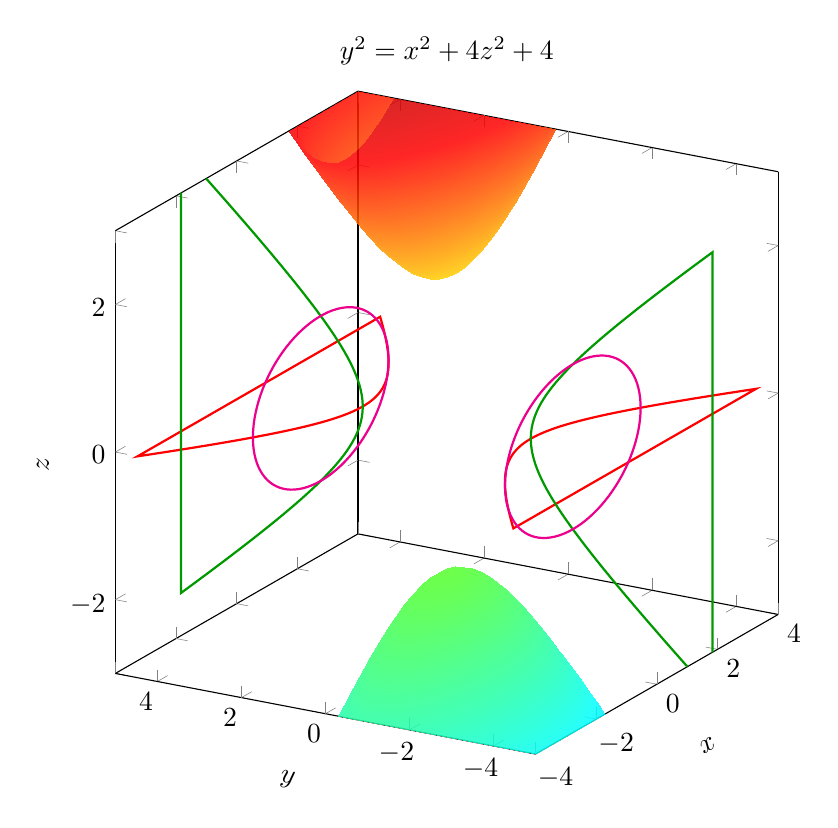
\begin{tikzpicture}
\begin{axis}[
    view={-60}{20},
    xlabel=$x$, ylabel=$y$, zlabel=$z$,
    xlabel style={sloped like x axis},
    ylabel style={sloped like y axis},
    zlabel style={sloped like z axis},
    xmin=-4, xmax=4,
    ymin=-5, ymax=5,
    zmin=-3, zmax=3,
    samples=30,
    samples y=30,
    colormap/bluered,
    title={$y^2=x^2+4z^2+4$},
    width=10cm, height=10cm
]
\addplot3[surf, shader=interp, domain=-4:4, y domain=-3:3, opacity=0.85] {2*sqrt(1+x^2/4+y^2)};
\addplot3[surf, shader=interp, domain=-4:4, y domain=-3:3, opacity=0.85] {-2*sqrt(1+x^2/4+y^2)};
% z=0 trace hyperbola
\addplot3[red, thick, domain=-4:4, samples=100, variable=\t] ({\t},{2*sqrt(1+\t^2/4)},0);
\addplot3[red, thick, domain=-4:4, samples=100, variable=\t] ({\t},{-2*sqrt(1+\t^2/4)},0);
% x=0 trace hyperbola
\addplot3[green!60!black, thick, domain=-3:3, samples=100, variable=\t] (0,{2*sqrt(1+\t^2)},\t);
\addplot3[green!60!black, thick, domain=-3:3, samples=100, variable=\t] (0,{-2*sqrt(1+\t^2)},\t);
% y=3 ellipse
\addplot3[magenta, thick, domain=0:360, samples=100, variable=\theta] ({2*sqrt(5/4)*cos(\theta)},3,{sqrt(5/4)*sin(\theta)});
\addplot3[magenta, thick, domain=0:360, samples=100, variable=\theta] ({2*sqrt(5/4)*cos(\theta)},-3,{sqrt(5/4)*sin(\theta)});
\end{axis}
\end{tikzpicture}
\end{document}
